% Define colors
\definecolor{headerColor}{HTML}{4F81BD}
\definecolor{rowColor1}{HTML}{B8CCE4}
\definecolor{rowColor2}{HTML}{DCE6F1}
\definecolor{textColor}{HTML}{000000}
\definecolor{highlightColor}{HTML}{00B0F0}
\section{Comparsion} 
\label{sec:3_6_comparsion}

This section presents a critical comparison of closely related works addressing the challenges of imbalanced multiclass streams \ref{sec:3_6_1_related_work_imbalanced}, the emergence of new classes \ref{sec:3_6_2_related_work_emergence}, and the integration of transfer learning \ref{sec:3_6_2_related_work_transfer} within streaming environments. The increasing complexity of real-world data streams necessitates advanced methodologies that can effectively manage the intricacies of these challenges. By examining various approaches in the literature, the goal is to highlight their contributions, strengths, and limitations in dealing with imbalanced data distributions, adapting to new class occurrences, and leveraging transfer learning techniques. This comparative analysis highlights the current state of research while emphasizing specific gaps and unresolved challenges, paving the way for more robust and adaptive solutions in streaming data classification.


\subsection{Imbalanced Stream}
\label{sec:3_6_1_related_work_imbalanced}

Addressing class imbalances is critical in multi-class classification. Multi-Label SMOTE (MLSMOTE) \cite{charte2015mlsmote} enhances classifier performance by generating synthetic examples for minority class labels using neighboring examples in the feature space. However, Multi-Label Synthetic Oversampling based on Local label imbalance (MLSOL) \cite{liu2022multi} improves upon this by employing tailored sampling strategies for each label to address local imbalances. Research shows that MLSOL outperforms MLSMOTE in classification accuracy and computational efficiency by generating synthetic samples from minority instances within restricted neighborhoods, resulting in a more compact and efficient dataset while reducing overfitting. Figure \ref{fig:mlsmote_mlsol} illustrates that MLSOL is more likely to select $x1$ as a seed instance because it is surrounded by more neighbors of the opposite class for $l3$. MLSMOTE assigns the label vector [0,1,0] to all synthetic instances based on their neighbors. In contrast, MLSOL creates more diverse instances by assigning labels according to their location. Moreover, synthetic instances $c2$ and $c3$ generated by MLSMOTE introduce noise, whereas MLSOL copies the labels of the nearest instance to the new examples. In summary, MLSMOTE tends to generate new instances biased toward the dominant class in the local area, whereas MLSOL effectively explores and exploits both the feature and label space.
\begin{figure*}[!ht]

    \begin{center}
      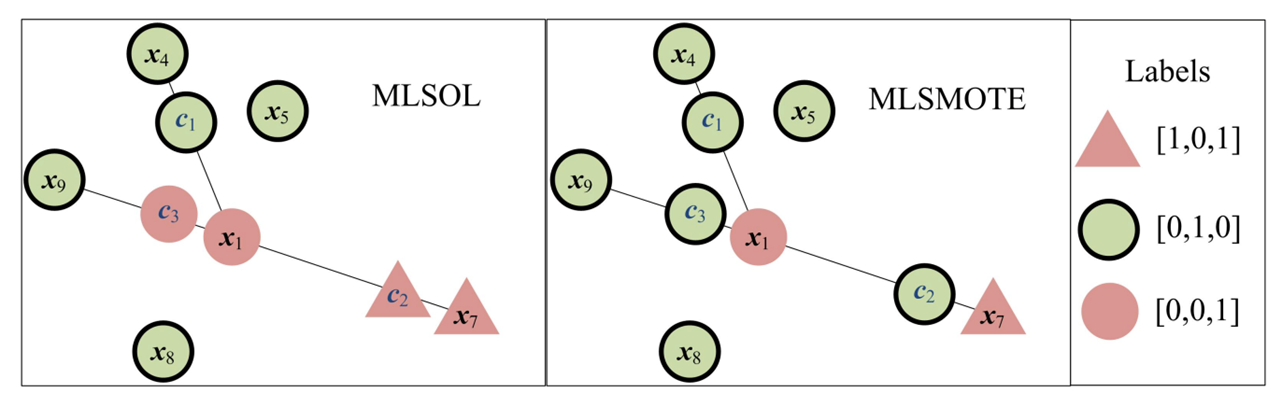
\includegraphics[width=1\textwidth]{3_State-of-the-art/fig/mlsmote_mlsol.png}
    \end{center}

    \caption{Comparsion of MLSMOTE and MLSOL Generated Instances \cite{liu2022multi}.\\ \textcolor{gray}{\fontsize{10}{0}\selectfont DOI: 110.1016/j.patcog.2021.108294}}
    \label{fig:mlsmote_mlsol}

    \end{figure*}
    
    Table \ref{table:imbalanced} compares MLSMOTE and MLSOL, two methods for addressing imbalanced data in multi-class classification. MLSMOTE generates synthetic examples for minority classes to balance distributions but may blur class distinctions and struggles with overlapping classes, leading to misclassification. MLSOL improves upon this by using localized sampling strategies to address local imbalances more effectively. However, both methods face limitations with overlapping class boundaries, which impact their overall classification accuracy. Despite MLSOL's precision in handling local imbalances, the challenge of overlapping classes remains significant for both approaches.
\begin{table*}[!ht]

    \centering
    \caption{Comparison of the MLSMOTE and MLSOL Methods.}
    \label{table:imbalanced}

    \small % Reduce font size
    \renewcommand{\arraystretch}{1} % Reduce cell padding
    \setlength{\tabcolsep}{4pt} % Reduce cell padding
    \setlength{\arrayrulewidth}{0.15mm}

    \begin{tabularx}{\textwidth}{|>{\centering\arraybackslash\bfseries}p{2cm}|
                                       >{\raggedright\arraybackslash}X|
                                       >{\raggedright\arraybackslash}X|
                                       >{\raggedright\arraybackslash}X|}
    \hline
    \textbf{Method} & \textbf{Theory} & \textbf{Advantages} & \textbf{Limitations} \\ 
    \hline
    \textbf{MLSMOTE \cite{charte2015mlsmote}} & 
    MLSMOTE significantly enhances classifier performance by generating synthetic examples for each minority class label. & 
    Generating synthetic examples for each minority class label. & 
    \begin{itemize}[leftmargin=*]
        \item Random synthetic samples may be related to the majority class.
        \item Overlapping classes.
    \end{itemize} \\ 
    \hline
    \textbf{MLSOL \cite{liu2022multi}} & 
    MLSOL systematically combats local imbalances within the domain of multi-class classification by employing distinct sampling strategies for each label. & 
    Generating synthetic examples for each minority class label within a restricted neighborhood. & 
    \begin{itemize}[leftmargin=*]
        \item Overlapping classes.
    \end{itemize} \\
    \hline
    \end{tabularx}
    \end{table*}

\subsection{Emergence of new classes}
\label{sec:3_6_2_related_work_emergence}


Detecting and adapting to new classes in streaming data is essential for maintaining classification accuracy. Tree-based methods like SENCForest \cite{mu2017classification} and SEEN \cite{zhu2020semi} use anomaly detection but suffer from high false positive rates and inefficiencies. SENNE improves detection using a nearest neighbor ensemble but has longer runtimes due to ineffective model retirement. The k-Nearest Neighbor Ensemble-based method (KNNENS) \cite{zhang2022knnens} enhances new class detection and known class classification through hypersphere ensembles and dynamic model updates. However, all these methods struggle to handle concept drift effectively, which is critical for detecting new classes and updating classification models.

Figures \ref{fig:SENCForest}, \ref{fig:SENNE}, and \ref{fig:KENNE} illustrate key approaches for classifying emerging and known classes. SENCForest divides the space into three regions (normal, outlying, and anomaly) and detects new classes using threshold path lengths. SENNE uses hyperplanes in three dimensions ($x1$, $x2$, and $x3$) to classify instances as emerging or known based on class rankings. KNNENS employs hyperplanes for all class samples and uses a voting mechanism to classify instances as emerging or known. These visualizations emphasize the differences in how SENNE and KNNENS handle class classification.

\begin{figure*}[!ht]
    \centering
    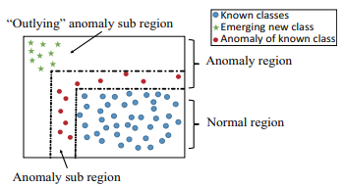
\includegraphics[width=0.80\textwidth]{3_State-of-the-art/fig/SENCForst.png}
    \caption{Overview of SENCForest Detection Flow Diagram \cite{mu2017classification}. \\
    \textcolor{gray}{\fontsize{10}{0}\selectfont DOI: 10.1109/TKDE.2017.2691702}}
    \label{fig:SENCForest}
\end{figure*}
    

\begin{figure*}[!ht]
    \begin{center}
        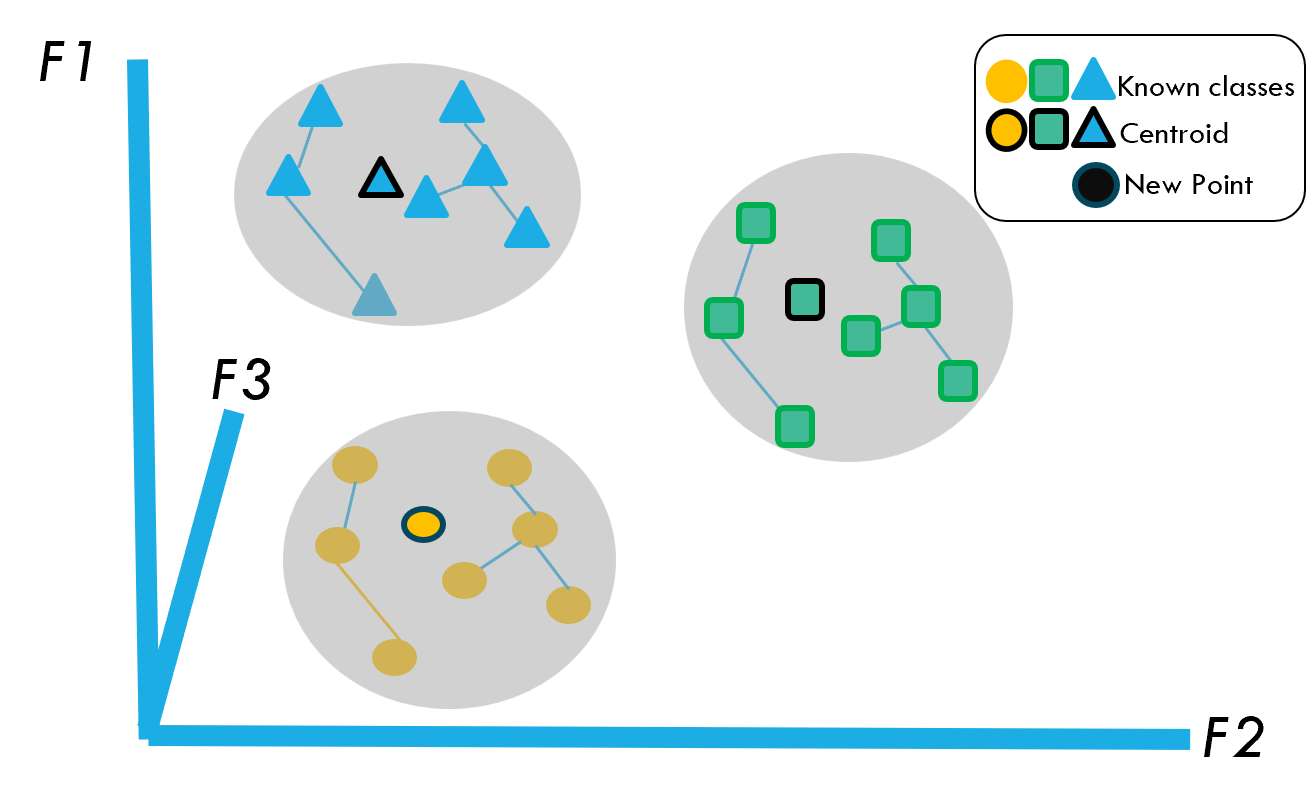
\includegraphics[width=.45\textwidth]{3_State-of-the-art/fig/senne0.png} 
        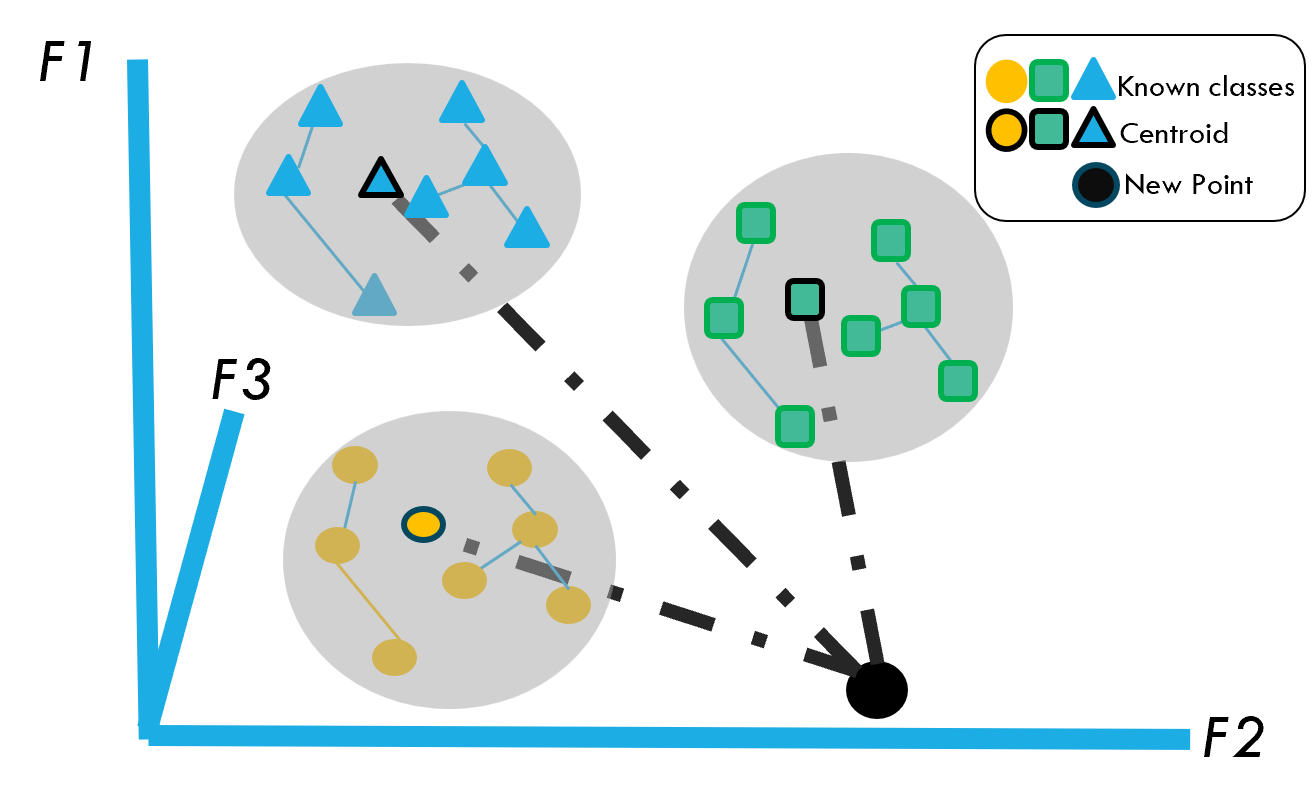
\includegraphics[width=.45\textwidth]{3_State-of-the-art/fig/senne.png} 
        (a)\hspace{6.5cm}(b)
    \end{center}
    \caption{Overview of the Stream Emerging Nearest Neighbor Ensemble (SENNE) \cite{zhu2020semi}.}
    \label{fig:SENNE}
    \end{figure*}
    \vline
    \begin{figure*}[!ht]    
        \begin{center}
            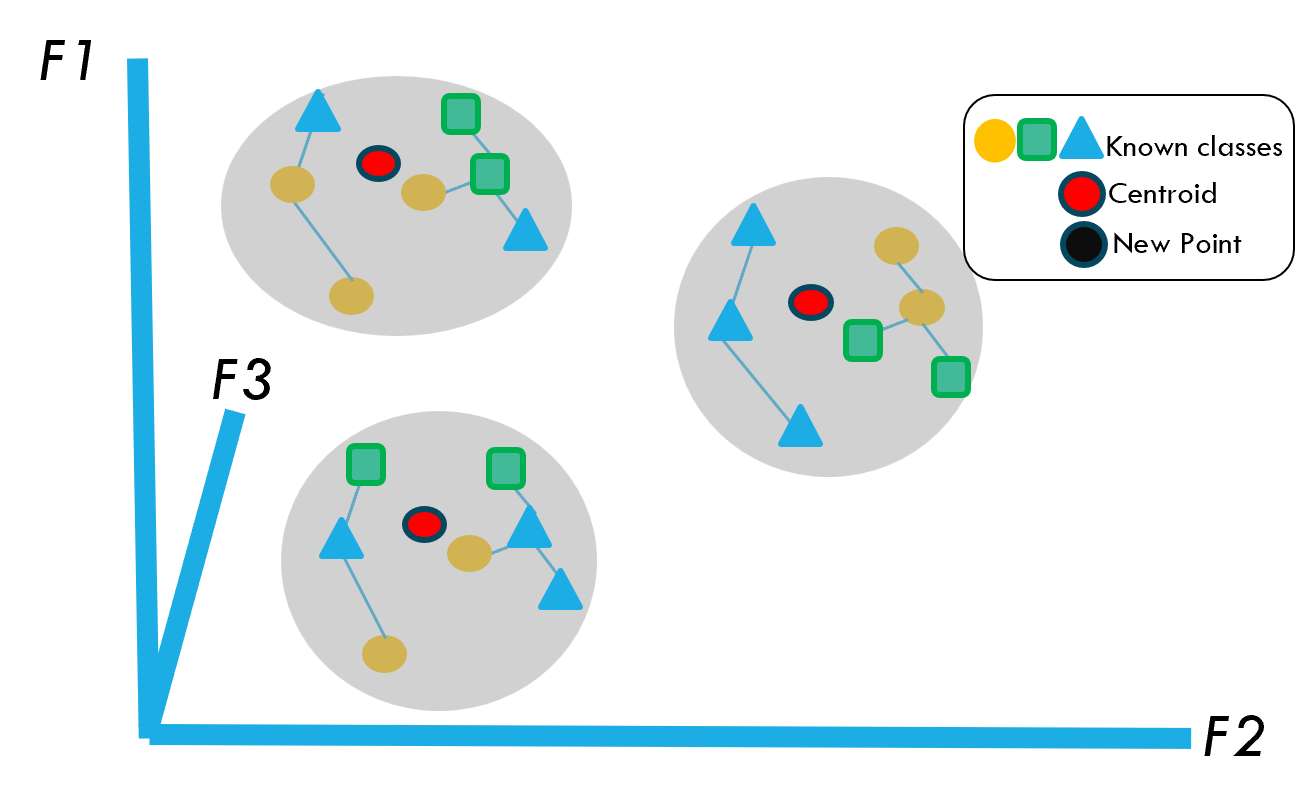
\includegraphics[width=.45\textwidth]{3_State-of-the-art/fig/kenne0.png} 
            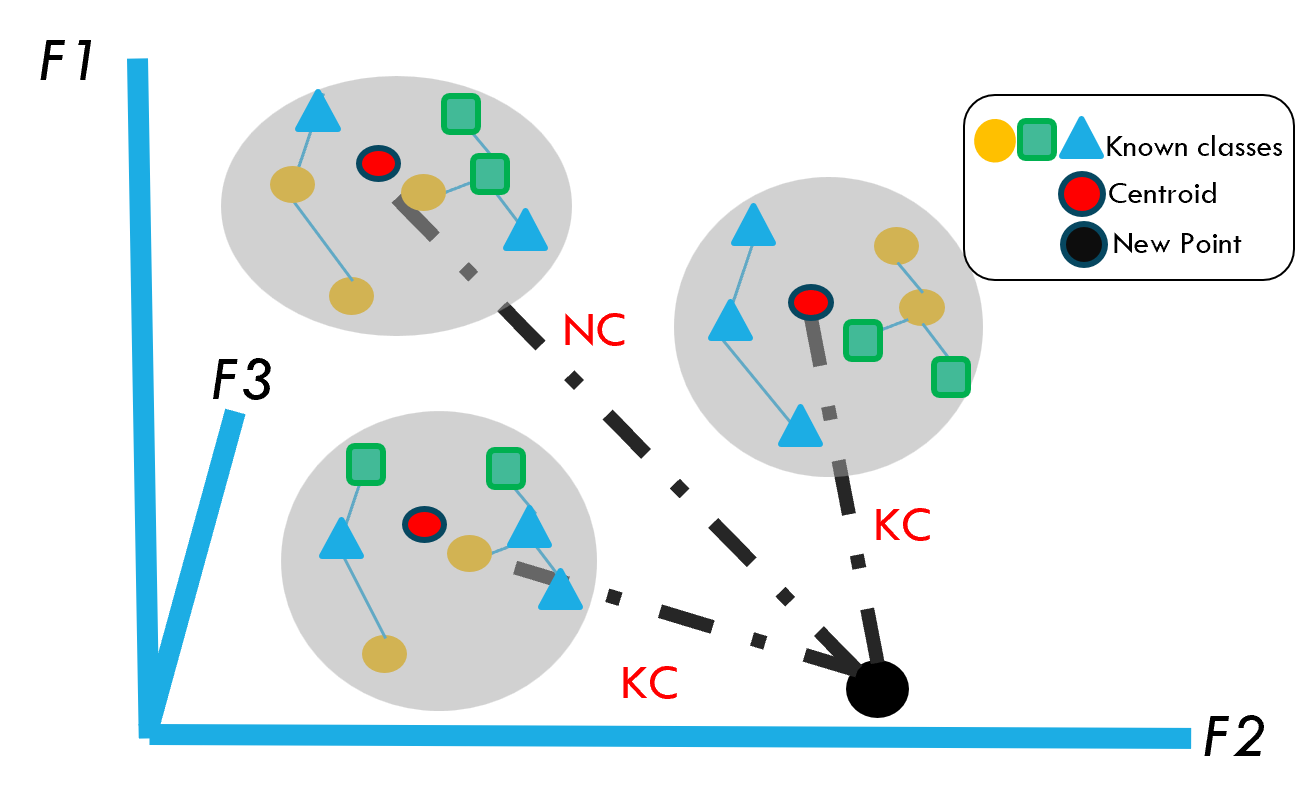
\includegraphics[width=.45\textwidth]{3_State-of-the-art/fig/kenne.png}
            (a)\hspace{6.5cm}(b)
            \end{center}
    
        \caption{Overview of the k-nearest Neighbor Ensemble-based \cite{zhang2022knnens} (KENNE).}
        \label{fig:KENNE}
        \end{figure*}
        
        Table \ref{table:emerging} compares three emerging class detection methods: SENCForest, SENNE, and KNNENS. SENCForest uses iForest \cite{wang2010negative} for anomaly detection and a threshold path for identifying new classes, serving as both an unsupervised detector and supervised classifier, but it is prone to false positives and relies on a complex threshold mechanism. SENNE utilizes a nearest neighbor-based hypersphere ensemble to analyze local neighborhood information, effectively handling varying geometric distances between classes, though it assumes static class distributions and has lengthy update times. KNNENS improves by using a hypersphere ensemble for all classes, reducing false positives and enabling updates without true labels, but it shares SENNE's limitation of assuming unchanged known class distributions.
\begin{table*}[!ht]

    \centering
    \caption{Comparison of the SENCForest, SENNE, and KENNE methods.}
    \label{table:emerging}
    \small % Reduce font size
    \renewcommand{\arraystretch}{1} % Reduce cell padding
    \setlength{\tabcolsep}{4pt} % Reduce cell padding
    \setlength{\arrayrulewidth}{0.15mm}
    \begin{tabularx}{\textwidth}{|>{\centering\arraybackslash\bfseries}p{2cm}|
                                       >{\raggedright\arraybackslash}X|
                                       >{\raggedright\arraybackslash}X|
                                       >{\raggedright\arraybackslash}X|}
    \hline
    \textbf{Method} & \textbf{Theory} & \textbf{Advantages} & \textbf{Limitations} \\ 
    \hline
    \textbf{SENCForst \cite{mu2017classification}} & 
    employs anomaly detection method iForest for a new class detection and then applies threshold path to detect the anomalies. & 
    SENCForest serves as both an unsupervised anomaly detector and a supervised classifier.&
    \begin{itemize}[leftmargin=*]
        \item Potential for High false positives.
        \item Dependency on path length threshold (more complexity).
    \end{itemize} \\ 
    \hline
    \textbf{SENNE \cite{zhu2020semi}} & 
    nearest neighbor-based hypersphere of one class ensemble to explore local neighborhood information and sort distance to calculate distance. & 
    SENNE is able to handle both the low and high geometric distance between two classes in the feature space. & 
    \begin{itemize}[leftmargin=*]
        \item Assumes that the distribution of known classes remains unchanged.
        \item Take long time for update.
    \end{itemize} \\ 
    \hline
    \textbf{KENNE \cite{zhang2022knnens}} & 
    nearest neighbor-based hypersphere of all class ensemble to explore local neighborhood information. & 
    KNNENS to reduce false positives for the new class. KNNENS does not require true labels to update the model. & 
    \begin{itemize}[leftmargin=*]
        \item Assumes that the distribution of known classes remains unchanged.
    \end{itemize} \\
    \hline
    \end{tabularx}
    \end{table*}



\subsection{Transfer Learning}
\label{sec:3_6_2_related_work_transfer}

In transfer learning, CORAL, Melanie, and HE-CDTL are key approaches related to the third proposed method \ref{chapter:6_transfer_learning}. CORAL \cite{sun2016return} aligns sub-space bases through second-order statistics using a learned transformation matrix, minimizing domain discrepancies and negative transfer. Melanie \cite{dong2019multistream} employs an online ensemble learning strategy to address non-stationary environments by incrementally training models from source and target domains, dynamically adjusting weights, and combining models via a weighted-sum approach. HE-CDTL extends these concepts specifically for Concept Drift Transfer Learning (CDTL), leveraging historical and source domain knowledge through a class-wise weighted ensemble and AW-CORAL to reduce domain disparities. Experiments show HE-CDTL outperforms baseline methods, demonstrating its efficacy in managing transfer learning under concept drift.
Table \ref{table:transfer} compares CORAL, Melanie, and HE-CDTL for transfer learning. CORAL minimizes domain discrepancies and reduces negative transfer by projecting source data into the target domain using a transformation matrix and Singular Value Decomposition (SVD) but struggles with non-stationary and heterogeneous data. Melanie addresses non-stationary environments in online learning by dynamically training and combining models from source and target domains, yet faces challenges with the complexity of online learning and data heterogeneity. HE-CDTL reduces domain shifts by aligning second-order statistics and leveraging historical knowledge but depends on source domain quality and also encounters issues with heterogeneous data.
\begin{figure*}[!ht]

    \begin{center}
        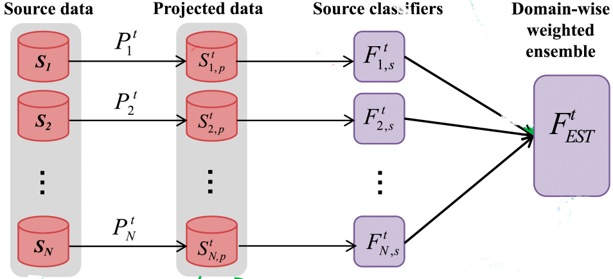
\includegraphics[width=.80\textwidth]{3_State-of-the-art/fig/coral.png} 
    \end{center}
    \caption{Overview of CORrelation ALignment (CORAL)\cite{sun2016return}.}
    \label{coral_fig}
    \end{figure*}
    \begin{figure*}[!ht]    
        \begin{center}
            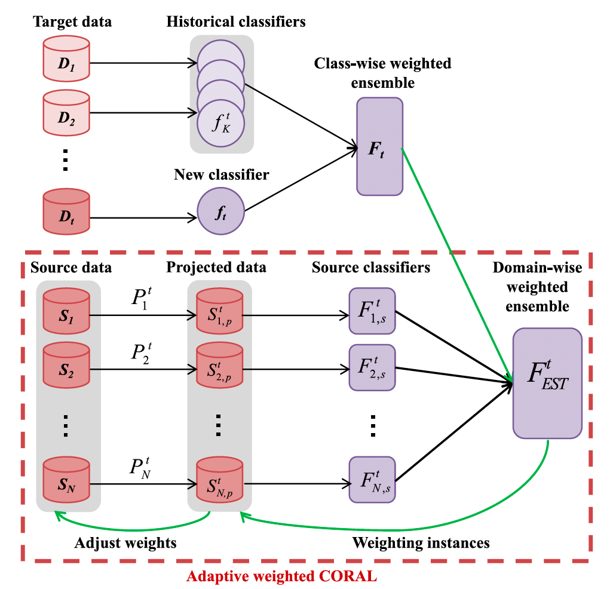
\includegraphics[width=.80\textwidth]{3_State-of-the-art/fig/cdtl.png} 
        \end{center}
        \caption{Overview of Concept Drift Transfer Learning (CDTL) \cite{sun2016return}.}
        \label{cdtl_fig}

        \end{figure*}

\begin{table*}[!ht]
    \centering
    \caption{Comparison of the CORAL, Malanie, and CDTL Methods.}
    \label{table:transfer}
    \small % Reduce font size
    \renewcommand{\arraystretch}{1} % Reduce cell padding
    \setlength{\tabcolsep}{4pt} % Reduce cell padding
    \setlength{\arrayrulewidth}{0.15mm}
    \begin{tabularx}{\textwidth}{|>{\centering\arraybackslash\bfseries}p{2cm}|
                                       >{\raggedright\arraybackslash}X|
                                       >{\raggedright\arraybackslash}X|
                                       >{\raggedright\arraybackslash}X|}
    \hline
    \textbf{Method} & \textbf{Theory} & \textbf{Advantages} & \textbf{Limitations} \\ 
    \hline
    \textbf{CORAL \cite{sun2016return}} & 
    Correlation Alignment (CORAL) uses a learned transformation matrix and Singular Value Decomposition (SVD)  to project the source instances into the target domain. & 
    CORAL can minimize domain discrepancy across
source and target domains, meanwhile reducing the negative
knowledge transfer. & 
    \begin{itemize}[leftmargin=*]
        \item Non-stationary environments.
        \item Heterogenous multisource.
    \end{itemize} \\ 
    \hline
    \textbf{Melanie \cite{dong2019multistream}} & 
    Multi-sourcE onLine TrAnsfer
learning for Non-statIonary Environments (Melanie). utilize the class-wise weighted . & 
It considers
an online problem in which the data in source and target
domains are generated from non-stationary environments. & 
    \begin{itemize}[leftmargin=*]
        \item Based on the online learning  only.
        \item Heterogenous multisource.
    \end{itemize} \\
    \hline
    \textbf{HE-CDTL \cite{sun2016return}} & 
    HE-CDTL uses the class-wise weighted and domain wise ensemble for historical knowledge and reduce the disparities between the source and target domains . & 
    HE-CDTL minimizes domain shift by aligning the second-order statistics of source and target distributions. & 
    \begin{itemize}[leftmargin=*]
        \item Depend on source domain quality.
        \item Heterogenous multisource.
    \end{itemize} \\
    \hline
    \end{tabularx}
    \end{table*}
